% Generated by Sphinx.
\def\sphinxdocclass{article}
\documentclass[a4paper,10pt,twocolumn,english]{sphinxsnamc2013}
\usepackage[utf8]{inputenc}
\DeclareUnicodeCharacter{00A0}{\nobreakspace}
\usepackage{cmap}
\usepackage[T1]{fontenc}
\usepackage[english]{babel}


\usepackage{longtable}
\usepackage{sphinx}
\usepackage{multirow}


% redefine title color (defined in sphinx style) to black:
%\definecolor{TitleColor}{rgb}{0.0,0.0,0.0}

%\usepackage{snamc2013}
\usepackage{fancyvrb}
\usepackage{graphicx}  % allows inclusion of graphics
\usepackage{booktabs}  % nice rules (thick lines) for tables
\usepackage{microtype} % improves typography for PDF

%\usepackage[breaklinks=true,colorlinks=true,linkcolor=black,citecolor=black]{hyperref}
%\usepackage{hypcap}

%\usepackage{courier}


\title{Python-based framework for coupled MC-TH reactor calculations}

\author[1]{Anton A. Travleev}
\author[1]{Richard Molitor}
\author[1]{Victor Sanchez}

\affil[1]{Institute for Neutron Physics and Reactor Technology (INR), Karlsruhe Institute of Technology,\newline%
Hermann-von-Helmholtz-Platz 1, 76344 Eggenstein-Leopoldshafen}

\abstract{%
We develop a set of Python packages to provide a modern programming interface
to codes used for analysis of nuclear reactors. Currently implemented
interfaces to the Monte Carlo (MC) neutronics code MCNP and thermo-hydraulic
(TH) code SCF allow efficient description of calculation models and provide a
framework for coupled calculations.

In this paper we illustrate how these interfaces can be used to describe a
pin model, and report results of coupled MCNP-SCF calculations performed 
for a PWR fuel assembly, organized by means of the interfaces.
}

\keywords{Python, MCNP, SCF, coupled MC-TH}




\makeatletter
\def\PYG@reset{\let\PYG@it=\relax \let\PYG@bf=\relax%
    \let\PYG@ul=\relax \let\PYG@tc=\relax%
    \let\PYG@bc=\relax \let\PYG@ff=\relax}
\def\PYG@tok#1{\csname PYG@tok@#1\endcsname}
\def\PYG@toks#1+{\ifx\relax#1\empty\else%
    \PYG@tok{#1}\expandafter\PYG@toks\fi}
\def\PYG@do#1{\PYG@bc{\PYG@tc{\PYG@ul{%
    \PYG@it{\PYG@bf{\PYG@ff{#1}}}}}}}
\def\PYG#1#2{\PYG@reset\PYG@toks#1+\relax+\PYG@do{#2}}

\expandafter\def\csname PYG@tok@gd\endcsname{\def\PYG@tc##1{\textcolor[rgb]{0.63,0.00,0.00}{##1}}}
\expandafter\def\csname PYG@tok@gu\endcsname{\let\PYG@bf=\textbf\def\PYG@tc##1{\textcolor[rgb]{0.50,0.00,0.50}{##1}}}
\expandafter\def\csname PYG@tok@gt\endcsname{\def\PYG@tc##1{\textcolor[rgb]{0.00,0.27,0.87}{##1}}}
\expandafter\def\csname PYG@tok@gs\endcsname{\let\PYG@bf=\textbf}
\expandafter\def\csname PYG@tok@gr\endcsname{\def\PYG@tc##1{\textcolor[rgb]{1.00,0.00,0.00}{##1}}}
\expandafter\def\csname PYG@tok@cm\endcsname{\let\PYG@it=\textit\def\PYG@tc##1{\textcolor[rgb]{0.25,0.50,0.56}{##1}}}
\expandafter\def\csname PYG@tok@vg\endcsname{\def\PYG@tc##1{\textcolor[rgb]{0.73,0.38,0.84}{##1}}}
\expandafter\def\csname PYG@tok@m\endcsname{\def\PYG@tc##1{\textcolor[rgb]{0.13,0.50,0.31}{##1}}}
\expandafter\def\csname PYG@tok@mh\endcsname{\def\PYG@tc##1{\textcolor[rgb]{0.13,0.50,0.31}{##1}}}
\expandafter\def\csname PYG@tok@cs\endcsname{\def\PYG@tc##1{\textcolor[rgb]{0.25,0.50,0.56}{##1}}\def\PYG@bc##1{\setlength{\fboxsep}{0pt}\colorbox[rgb]{1.00,0.94,0.94}{\strut ##1}}}
\expandafter\def\csname PYG@tok@ge\endcsname{\let\PYG@it=\textit}
\expandafter\def\csname PYG@tok@vc\endcsname{\def\PYG@tc##1{\textcolor[rgb]{0.73,0.38,0.84}{##1}}}
\expandafter\def\csname PYG@tok@il\endcsname{\def\PYG@tc##1{\textcolor[rgb]{0.13,0.50,0.31}{##1}}}
\expandafter\def\csname PYG@tok@go\endcsname{\def\PYG@tc##1{\textcolor[rgb]{0.20,0.20,0.20}{##1}}}
\expandafter\def\csname PYG@tok@cp\endcsname{\def\PYG@tc##1{\textcolor[rgb]{0.00,0.44,0.13}{##1}}}
\expandafter\def\csname PYG@tok@gi\endcsname{\def\PYG@tc##1{\textcolor[rgb]{0.00,0.63,0.00}{##1}}}
\expandafter\def\csname PYG@tok@gh\endcsname{\let\PYG@bf=\textbf\def\PYG@tc##1{\textcolor[rgb]{0.00,0.00,0.50}{##1}}}
\expandafter\def\csname PYG@tok@ni\endcsname{\let\PYG@bf=\textbf\def\PYG@tc##1{\textcolor[rgb]{0.84,0.33,0.22}{##1}}}
\expandafter\def\csname PYG@tok@nl\endcsname{\let\PYG@bf=\textbf\def\PYG@tc##1{\textcolor[rgb]{0.00,0.13,0.44}{##1}}}
\expandafter\def\csname PYG@tok@nn\endcsname{\let\PYG@bf=\textbf\def\PYG@tc##1{\textcolor[rgb]{0.05,0.52,0.71}{##1}}}
\expandafter\def\csname PYG@tok@no\endcsname{\def\PYG@tc##1{\textcolor[rgb]{0.38,0.68,0.84}{##1}}}
\expandafter\def\csname PYG@tok@na\endcsname{\def\PYG@tc##1{\textcolor[rgb]{0.25,0.44,0.63}{##1}}}
\expandafter\def\csname PYG@tok@nb\endcsname{\def\PYG@tc##1{\textcolor[rgb]{0.00,0.44,0.13}{##1}}}
\expandafter\def\csname PYG@tok@nc\endcsname{\let\PYG@bf=\textbf\def\PYG@tc##1{\textcolor[rgb]{0.05,0.52,0.71}{##1}}}
\expandafter\def\csname PYG@tok@nd\endcsname{\let\PYG@bf=\textbf\def\PYG@tc##1{\textcolor[rgb]{0.33,0.33,0.33}{##1}}}
\expandafter\def\csname PYG@tok@ne\endcsname{\def\PYG@tc##1{\textcolor[rgb]{0.00,0.44,0.13}{##1}}}
\expandafter\def\csname PYG@tok@nf\endcsname{\def\PYG@tc##1{\textcolor[rgb]{0.02,0.16,0.49}{##1}}}
\expandafter\def\csname PYG@tok@si\endcsname{\let\PYG@it=\textit\def\PYG@tc##1{\textcolor[rgb]{0.44,0.63,0.82}{##1}}}
\expandafter\def\csname PYG@tok@s2\endcsname{\def\PYG@tc##1{\textcolor[rgb]{0.25,0.44,0.63}{##1}}}
\expandafter\def\csname PYG@tok@vi\endcsname{\def\PYG@tc##1{\textcolor[rgb]{0.73,0.38,0.84}{##1}}}
\expandafter\def\csname PYG@tok@nt\endcsname{\let\PYG@bf=\textbf\def\PYG@tc##1{\textcolor[rgb]{0.02,0.16,0.45}{##1}}}
\expandafter\def\csname PYG@tok@nv\endcsname{\def\PYG@tc##1{\textcolor[rgb]{0.73,0.38,0.84}{##1}}}
\expandafter\def\csname PYG@tok@s1\endcsname{\def\PYG@tc##1{\textcolor[rgb]{0.25,0.44,0.63}{##1}}}
\expandafter\def\csname PYG@tok@gp\endcsname{\let\PYG@bf=\textbf\def\PYG@tc##1{\textcolor[rgb]{0.78,0.36,0.04}{##1}}}
\expandafter\def\csname PYG@tok@sh\endcsname{\def\PYG@tc##1{\textcolor[rgb]{0.25,0.44,0.63}{##1}}}
\expandafter\def\csname PYG@tok@ow\endcsname{\let\PYG@bf=\textbf\def\PYG@tc##1{\textcolor[rgb]{0.00,0.44,0.13}{##1}}}
\expandafter\def\csname PYG@tok@sx\endcsname{\def\PYG@tc##1{\textcolor[rgb]{0.78,0.36,0.04}{##1}}}
\expandafter\def\csname PYG@tok@bp\endcsname{\def\PYG@tc##1{\textcolor[rgb]{0.00,0.44,0.13}{##1}}}
\expandafter\def\csname PYG@tok@c1\endcsname{\let\PYG@it=\textit\def\PYG@tc##1{\textcolor[rgb]{0.25,0.50,0.56}{##1}}}
\expandafter\def\csname PYG@tok@kc\endcsname{\let\PYG@bf=\textbf\def\PYG@tc##1{\textcolor[rgb]{0.00,0.44,0.13}{##1}}}
\expandafter\def\csname PYG@tok@c\endcsname{\let\PYG@it=\textit\def\PYG@tc##1{\textcolor[rgb]{0.25,0.50,0.56}{##1}}}
\expandafter\def\csname PYG@tok@mf\endcsname{\def\PYG@tc##1{\textcolor[rgb]{0.13,0.50,0.31}{##1}}}
\expandafter\def\csname PYG@tok@err\endcsname{\def\PYG@bc##1{\setlength{\fboxsep}{0pt}\fcolorbox[rgb]{1.00,0.00,0.00}{1,1,1}{\strut ##1}}}
\expandafter\def\csname PYG@tok@kd\endcsname{\let\PYG@bf=\textbf\def\PYG@tc##1{\textcolor[rgb]{0.00,0.44,0.13}{##1}}}
\expandafter\def\csname PYG@tok@ss\endcsname{\def\PYG@tc##1{\textcolor[rgb]{0.32,0.47,0.09}{##1}}}
\expandafter\def\csname PYG@tok@sr\endcsname{\def\PYG@tc##1{\textcolor[rgb]{0.14,0.33,0.53}{##1}}}
\expandafter\def\csname PYG@tok@mo\endcsname{\def\PYG@tc##1{\textcolor[rgb]{0.13,0.50,0.31}{##1}}}
\expandafter\def\csname PYG@tok@mi\endcsname{\def\PYG@tc##1{\textcolor[rgb]{0.13,0.50,0.31}{##1}}}
\expandafter\def\csname PYG@tok@kn\endcsname{\let\PYG@bf=\textbf\def\PYG@tc##1{\textcolor[rgb]{0.00,0.44,0.13}{##1}}}
\expandafter\def\csname PYG@tok@o\endcsname{\def\PYG@tc##1{\textcolor[rgb]{0.40,0.40,0.40}{##1}}}
\expandafter\def\csname PYG@tok@kr\endcsname{\let\PYG@bf=\textbf\def\PYG@tc##1{\textcolor[rgb]{0.00,0.44,0.13}{##1}}}
\expandafter\def\csname PYG@tok@s\endcsname{\def\PYG@tc##1{\textcolor[rgb]{0.25,0.44,0.63}{##1}}}
\expandafter\def\csname PYG@tok@kp\endcsname{\def\PYG@tc##1{\textcolor[rgb]{0.00,0.44,0.13}{##1}}}
\expandafter\def\csname PYG@tok@w\endcsname{\def\PYG@tc##1{\textcolor[rgb]{0.73,0.73,0.73}{##1}}}
\expandafter\def\csname PYG@tok@kt\endcsname{\def\PYG@tc##1{\textcolor[rgb]{0.56,0.13,0.00}{##1}}}
\expandafter\def\csname PYG@tok@sc\endcsname{\def\PYG@tc##1{\textcolor[rgb]{0.25,0.44,0.63}{##1}}}
\expandafter\def\csname PYG@tok@sb\endcsname{\def\PYG@tc##1{\textcolor[rgb]{0.25,0.44,0.63}{##1}}}
\expandafter\def\csname PYG@tok@k\endcsname{\let\PYG@bf=\textbf\def\PYG@tc##1{\textcolor[rgb]{0.00,0.44,0.13}{##1}}}
\expandafter\def\csname PYG@tok@se\endcsname{\let\PYG@bf=\textbf\def\PYG@tc##1{\textcolor[rgb]{0.25,0.44,0.63}{##1}}}
\expandafter\def\csname PYG@tok@sd\endcsname{\let\PYG@it=\textit\def\PYG@tc##1{\textcolor[rgb]{0.25,0.44,0.63}{##1}}}

\def\PYGZbs{\char`\\}
\def\PYGZus{\char`\_}
\def\PYGZob{\char`\{}
\def\PYGZcb{\char`\}}
\def\PYGZca{\char`\^}
\def\PYGZam{\char`\&}
\def\PYGZlt{\char`\<}
\def\PYGZgt{\char`\>}
\def\PYGZsh{\char`\#}
\def\PYGZpc{\char`\%}
\def\PYGZdl{\char`\$}
\def\PYGZhy{\char`\-}
\def\PYGZsq{\char`\'}
\def\PYGZdq{\char`\"}
\def\PYGZti{\char`\~}
% for compatibility with earlier versions
\def\PYGZat{@}
\def\PYGZlb{[}
\def\PYGZrb{]}
\makeatother

\begin{document}






\section{Introduction}
\label{paper:introduction}\label{paper::doc}\label{paper:main-entry}
The HPMC project \cite{hpmc} aims full-core coupled calculations
including Monte Carlo (MC) neutronics, thermo-hydraulics (TH), burnup and time dependence.  This goal
will be achieved in steps, starting from coupling two physics domains (e.g.
neutronics and thermo-hydraulics, neutronics and nuclide kinetics, etc.) for
simple pin and assembly geometries and gradually increasing complexity. It is
assumed in the HPMC project that on certain stage cluster computers will be
used for MC neutronics calculations.

These two aspects of the project imply that the coupling procedure need to
be reusable for different types of problems (like pin, assembly and whole core
models) and should be flexibly applied on different types of computers (like
small desktop machines and supercomputers).

Coupled neutronics -- TH calculations are widely used in reactor engineering and several
different approaches have been established to couple neutronics and TH codes. The
fastest in implementation approach to organize data flow between two particular
N and TH codes is to prepare input file templates and to write an interface
program (this approach is followed, for example,  in
\cite{HoogenboomMC2011}).  The interface program reads output from
one code, prepares data for the other code and inserts them into the correspondent
input file template. Both templates and the interface program are usually
written considering particular geometry type, which on the one hand
simplifies coding, but on the other hand makes it difficult to reuse the
coupling scheme for a different type of geometry.

Another way to couple neutronics and TH codes is to use a common platform
that provides means to integrate codes and to organize data flow between
them.  An example of this approach is the NURESIM system
\cite{nuresimICONE2006,nuresimWEB} that utilizes the SALOME
platform \cite{salomeWEB}. This approach results in much more
flexible solution as compared to the approach described above, but also has
some drawbacks. For example, integration of a code into the platform might
require changes in the code itself, which is not always possible due to e.g.
licensing limitations. Moreover, requirements to computer (hardware and OS) imposed by
SALOME are quite restrictive \cite{salomeWEB}.

In the present work we propose a coupling approach that can be applied to
different types of calculation geometry and does not require changes in the
code to be integrated. This approach is implemented as a set of Python
\cite{pythonWEB} packages called PIRS -- Python Interfaces for
Reactor Simulations that currently provides interfaces to MCNP
\cite{mcnpREF} and SCF codes \cite{scfREF}.

In this paper we describe  the concept of PIRS, give an example of neutronics
specifications for a simplified pin model, and report results of coupled
MCNP-SCF calculations for a PWR assembly organized by means of PIRS.


\section{Concept of the coupling framework}
\label{paper:concept-of-the-coupling-framework}
Python classes provided by PIRS can be classified by their functionality into
three groups: low-level interfaces, general model classes and high-level
interfaces, see figure \ref{pic:classes}.  Classes of the first
group describe an interface between Python and a particular code (low-level
interfaces). A low-level interface class allows to set any parameter in the
input file, generates it, provides means to execute the code and defines
procedures to read output files directly from the Python interpreter or a
Python script. Low-level classes ensure that the generated input files have
correct syntax and often saves a user from specifying auxiliary or non-used
parameters.
\begin{figure}[htbp]
\centering
\capstart

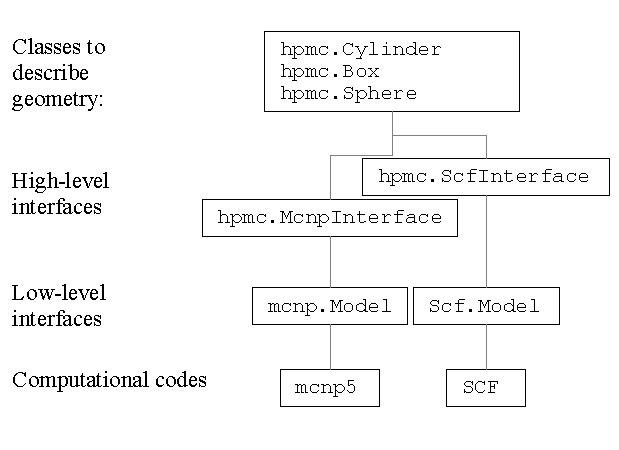
\includegraphics{scheme_en.pdf}
\caption{PIRS Classes and their interaction with computational codes. \label{pic:classes}}\end{figure}

General model classes can be used to describe calculation geometry and
meshes to represent system variables.

High-level interface classes are used to convert geometry described with general
model classes to instances of low-level interface classes and to put results
of code calculations (read by low-interface classes) back to general model.

To organize coupled neutronics -- TH calculations, a user defines parameters, common to
both neutronics and TH domains, in a variable (say, \code{a1}) by means of general model
classes. This variable contains information about geometry and axial
meshes for heat deposition, temperature and density. An instance of one of the
high-level interfaces (let call it \code{i1}) is used to set
code-specific information, like cross-sections data sets for MCNP. Variable
\code{i1} has a method that takes \code{a1} as an input model, prepares an input file
based on the common information stored in \code{a1} and code-specific data stored
in \code{i1}, executes the code, reads the code output and returns \code{a2} that is
a copy of \code{a1} except some system variables which are replaced with the results of
calculations. Variable \code{a2} can be passed to a high-level interface of
another code as the input model; in this way one can organize data flow between
codes. A user can arbitrarily change parameters of a model, e.g. to describe a
relaxation scheme.

This framework structure allows to develop independently code back ends (i.e.
low-level and high-level classes for a code), once the structure of the classes
representing general model is defined.


\section{Example: a simplified pin model}
\label{paper:example-a-simplified-pin-model}
A simplified pin model is considered to illustrate steps necessary to perform
neutronics calculations. First, a geometry of a model is described using general model
classes, and second, MCNP-specific date are specified with the help of
the MCNP high-level interface.


\subsection{Calculation geometry}
\label{paper:calculation-geometry}
The simplified pin model consists of two regions: a vertical cylinder (fuel) is
immersed into a rectangular parallelepiped (moderator). The following Python
script defines this model:

\begin{Verbatim}[commandchars=\\\{\}]
\PYG{k+kn}{from} \PYG{n+nn}{hpmc} \PYG{k+kn}{import} \PYG{n}{Box}\PYG{p}{,} \PYG{n}{Cylinder}

\PYG{n}{b} \PYG{o}{=} \PYG{n}{Box}\PYG{p}{(}\PYG{n}{X}\PYG{o}{=}\PYG{l+m+mf}{1.2}\PYG{p}{,} \PYG{n}{Y}\PYG{o}{=}\PYG{l+m+mf}{1.2}\PYG{p}{,} \PYG{n}{Z}\PYG{o}{=}\PYG{l+m+mi}{110}\PYG{p}{)}
\PYG{n}{c} \PYG{o}{=} \PYG{n}{Cylinder}\PYG{p}{(}\PYG{n}{R}\PYG{o}{=}\PYG{l+m+mf}{0.5}\PYG{p}{,} \PYG{n}{Z}\PYG{o}{=}\PYG{l+m+mi}{100}\PYG{p}{)}
\PYG{n}{b}\PYG{o}{.}\PYG{n}{insert}\PYG{p}{(}\PYG{l+m+mi}{0}\PYG{p}{,} \PYG{n}{c}\PYG{p}{)}

\PYG{n}{b}\PYG{o}{.}\PYG{n}{material} \PYG{o}{=} \PYG{l+s}{\PYGZsq{}}\PYG{l+s}{water}\PYG{l+s}{\PYGZsq{}}
\PYG{n}{c}\PYG{o}{.}\PYG{n}{material} \PYG{o}{=} \PYG{l+s}{\PYGZsq{}}\PYG{l+s}{fuel}\PYG{l+s}{\PYGZsq{}}

\PYG{n}{b}\PYG{o}{.}\PYG{n}{dens}\PYG{o}{.}\PYG{n}{set\PYGZus{}grid}\PYG{p}{(}\PYG{p}{[}\PYG{l+m+mi}{1}\PYG{p}{,} \PYG{l+m+mi}{1}\PYG{p}{]}\PYG{p}{)}
\PYG{n}{b}\PYG{o}{.}\PYG{n}{dens}\PYG{o}{.}\PYG{n}{set\PYGZus{}values}\PYG{p}{(}\PYG{l+m+mf}{1.}\PYG{p}{)}

\PYG{n}{c}\PYG{o}{.}\PYG{n}{temp}\PYG{o}{.}\PYG{n}{set\PYGZus{}grid}\PYG{p}{(}\PYG{p}{[}\PYG{l+m+mi}{1}\PYG{p}{]}\PYG{o}{*}\PYG{l+m+mi}{3}\PYG{p}{)}
\PYG{n}{c}\PYG{o}{.}\PYG{n}{temp}\PYG{o}{.}\PYG{n}{set\PYGZus{}values}\PYG{p}{(}\PYG{p}{[}\PYG{l+m+mi}{300}\PYG{p}{,} \PYG{l+m+mi}{500}\PYG{p}{,} \PYG{l+m+mi}{350}\PYG{p}{]}\PYG{p}{)}

\PYG{n}{c}\PYG{o}{.}\PYG{n}{heat}\PYG{o}{.}\PYG{n}{set\PYGZus{}grid}\PYG{p}{(}\PYG{p}{[}\PYG{l+m+mi}{1}\PYG{p}{]}\PYG{o}{*}\PYG{l+m+mi}{10}\PYG{p}{)}
\end{Verbatim}

The \code{Cylinder} and \code{Box} classes are imported from the \code{hpmc} module provided by PIRS.
These classes are used to set the geometrical elements --
constituents of the pin model.  Variable \code{b} is an instance of the \code{Box}
class; it describes a rectangular parallelepiped with sides 1.2 x 1.2 x 110
cm. Variable \code{c} is an instance of the \code{Cylinder} class and represents a
vertical cylinder with radius 0.5 cm and height 100 cm. The \code{insert} method of
variable \code{b} is used to specify positional relationship between solids \code{b}
and \code{c}: cylinder \code{c} is inserted into box \code{b}. Coordinates of \code{c} with
respect to \code{b} are not given explicitly and by default \code{c} is centered
with respect to \code{b}.

A material name can be given to each model's element, by means of the \code{material}
attribute.  This attribute is set by default  to \code{'void'} and can take
any string value.  Actual meaning of the material name must be defined for each
code using correspondent high-level interface.

Next, meshes to represent system variables are defined. Attributes \code{dens},
\code{temp} and \code{heat} represent density, temperature and heat deposition axial
distributions for each model's element, respectively. In the example above,
density of the element \code{b} is represented by an axial mesh with two equidistant
mesh elements; in both mesh elements density is set to 1.  Temperature of the element \code{c} is given by
an axial mesh with three equidistant mesh elements, temperatures are 300 K in the
lower mesh element, 500 K in the middle element and 350 K in the upper mesh
element. Additionally we specified that heat deposition should be represented by an axial
mesh with 10 equidistant elements, but no values are given explicitly.


\subsection{high-level interface to MCNP}
\label{paper:high-level-interface-to-mcnp}
The above script describes only geometry of the model. MCNP-specific data are
specified by means of the \code{MCNPInterface} class from the \code{hpmc} module.
This includes specification of material isotopic compositions, boundary
conditions and neutron source for criticality calculations.

\begin{Verbatim}[commandchars=\\\{\}]
\PYG{k+kn}{from} \PYG{n+nn}{hpmc} \PYG{k+kn}{import} \PYG{n}{McnpInterface}
\PYG{k+kn}{from} \PYG{n+nn}{mcnp} \PYG{k+kn}{import} \PYG{n}{Material}

\PYG{n}{m} \PYG{o}{=} \PYG{n}{McnpInterface}\PYG{p}{(}\PYG{n}{b}\PYG{p}{)}

\PYG{n}{u} \PYG{o}{=} \PYG{n}{Material}\PYG{p}{(}\PYG{p}{(}\PYG{l+m+mi}{92235}\PYG{p}{,}  \PYG{l+m+mf}{0.5}\PYG{p}{,} \PYG{l+m+mi}{2}\PYG{p}{)}\PYG{p}{,}
             \PYG{p}{(}\PYG{l+m+mi}{92238}\PYG{p}{,} \PYG{l+m+mf}{95.5}\PYG{p}{,} \PYG{l+m+mi}{2}\PYG{p}{)}\PYG{p}{)}

\PYG{n}{o} \PYG{o}{=} \PYG{n}{Material}\PYG{p}{(}\PYG{l+s}{\PYGZsq{}}\PYG{l+s}{O}\PYG{l+s}{\PYGZsq{}}\PYG{p}{)}             
\PYG{n}{h} \PYG{o}{=} \PYG{n}{Material}\PYG{p}{(}\PYG{l+s}{\PYGZsq{}}\PYG{l+s}{H}\PYG{l+s}{\PYGZsq{}}\PYG{p}{)}

\PYG{n}{f} \PYG{o}{=} \PYG{n}{u} \PYG{o}{+} \PYG{l+m+mi}{2}\PYG{o}{*}\PYG{n}{o}
\PYG{n}{w} \PYG{o}{=} \PYG{n}{h}\PYG{o}{*}\PYG{l+m+mi}{2} \PYG{o}{+} \PYG{n}{o}
\PYG{n}{w}\PYG{o}{.}\PYG{n}{thermal} \PYG{o}{=} \PYG{l+s}{\PYGZsq{}}\PYG{l+s}{lwtr}\PYG{l+s}{\PYGZsq{}}

\PYG{n}{f}\PYG{o}{.}\PYG{n}{sdict}\PYG{p}{[}\PYG{l+m+mi}{8018}\PYG{p}{]} \PYG{o}{=} \PYG{l+m+mi}{8016}
\PYG{n}{w}\PYG{o}{.}\PYG{n}{sdict}\PYG{p}{[}\PYG{l+m+mi}{8018}\PYG{p}{]} \PYG{o}{=} \PYG{l+m+mi}{8016}

\PYG{n}{m}\PYG{o}{.}\PYG{n}{materials}\PYG{p}{[}\PYG{l+s}{\PYGZsq{}}\PYG{l+s}{fuel}\PYG{l+s}{\PYGZsq{}}\PYG{p}{]} \PYG{o}{=} \PYG{n}{f}
\PYG{n}{m}\PYG{o}{.}\PYG{n}{materials}\PYG{p}{[}\PYG{l+s}{\PYGZsq{}}\PYG{l+s}{water}\PYG{l+s}{\PYGZsq{}}\PYG{p}{]} \PYG{o}{=} \PYG{n}{w}

\PYG{n}{m}\PYG{o}{.}\PYG{n}{bc}\PYG{p}{[}\PYG{l+s}{\PYGZsq{}}\PYG{l+s}{radial}\PYG{l+s}{\PYGZsq{}}\PYG{p}{]} \PYG{o}{=} \PYG{l+s}{\PYGZsq{}}\PYG{l+s}{*}\PYG{l+s}{\PYGZsq{}}

\PYG{n}{m}\PYG{o}{.}\PYG{n}{adc}\PYG{o}{.}\PYG{n}{append}\PYG{p}{(}\PYG{l+s}{\PYGZsq{}}\PYG{l+s}{ksrc 0 0 0}\PYG{l+s}{\PYGZsq{}}\PYG{p}{)}
\PYG{n}{m}\PYG{o}{.}\PYG{n}{adc}\PYG{o}{.}\PYG{n}{append}\PYG{p}{(}\PYG{l+s}{\PYGZsq{}}\PYG{l+s}{kcode 500 1. 20 100}\PYG{l+s}{\PYGZsq{}}\PYG{p}{)}

\PYG{n}{m}\PYG{o}{.}\PYG{n}{run}\PYG{p}{(}\PYG{l+s}{\PYGZsq{}}\PYG{l+s}{P}\PYG{l+s}{\PYGZsq{}}\PYG{p}{)}

\PYG{n}{r} \PYG{o}{=} \PYG{n}{m}\PYG{o}{.}\PYG{n}{run}\PYG{p}{(}\PYG{l+s}{\PYGZsq{}}\PYG{l+s}{R}\PYG{l+s}{\PYGZsq{}}\PYG{p}{)}
\end{Verbatim}

The \code{m} variable is an instance of the \code{McnpInterface} class; its
constructor takes optionally a variable representing general model (in this
example, the variable \code{b} defined earlier). Any geometry described using
\code{Cylinder} and \code{Box} classes and their arbitrary combinations can be
handled (understood) by the MCNP interface.

The \code{Material} class imported from the \code{mcnp} module (this module describes
low-level interface to MCNP) is used to define material compositions. Variables
\code{u}, \code{o} and \code{h} represent isotopic compositions of chemical elements
uranium, oxygen and hydrogen. Uranium
isotopic composition is given in weight fractions, for oxygen and hydrogen
natural abundance data \cite{natAbund2011} are used. Arithmetical
operations for instances of the \code{Material} class are defined in the way that
can be used to define new mixtures. In the example, variable \code{f} is a mixture
of 1 atomic part of uranium and two atomic parts of oxygen and represents
uranium dioxide.  The \code{w} variable represents water. Optionally, one can
specify a string pattern that will be used to find cross-section data for
thermal scattering, see the \code{thermal} attribute. In the example, thermal data
set for water will be chosen among thermal data sets with names containing
\code{'lwtr'} string with the closest temperature.

Materials \code{f} and \code{w} contain all
stable isotopes of oxygen, among them isotope 8018. In the
cross-section data set applied implicitly in this example, there is no data for
this isotope. To handle such situations, there is the \code{sdict} attribute of the
dictionary class that defines a substitution table: if for a given isotope (in
our example 8018) there is no cross-section, it is substituted with another one
(in our example 8016).

Correspondence between material compositions and general model material names
is defined in the attribute \code{materials}. It is a dictionary with
material names as keys and instances of the \code{Material} class as values.

Boundary conditions are set up using the \code{bc} attribute. It is an instance of
a dictionary-based class that admits only two keys, \code{radial} and \code{axial}.
By default, the values are empty strings meaning no reflection on radial and
axial general model outer boundaries. One can set them alternatively to \code{'*'}
or  \code{'+'} which means reflective or white boundary conditions, respectively
(similar to MCNP syntax). In the example we specify reflective radial boundary
conditions (for our model, the radial boundaries are the boundaries of the
water box that are perpendicular to the vertical axis) and leave default axial
boundary conditions.

Currently, there is no high-level interface to specify neutron source
parameters for an MCNP problem. As a workaround, a user can use possibility to
specify directly lines for the input file, provided by the low-level MCNP
interface. Attributes \code{adc}, \code{asc}, \code{acc} and \code{amc} are lists of lines that will
be appended to the data cards block, surface cards block, cell cards block and message cards
block, respectively. In the example we append two lines to the data cards
block, specifying initial spatial distribution of fission neutrons and
parameters of criticality calculations.

The \code{run} method generates the MCNP input file and starts the code. The first
call to the \code{run} method, with \code{'P'} argument, starts MCNP in the
geometry plotter mode.  In the second call with \code{'R'} argument, MCNP is
started in the particle transport mode. In this mode the interface waits until
MCNP finishes, reads heat deposition computed by mesh tallies and returns a
copy of the general model with heat attributes containing MCNP
results. Heat deposition mesh tallies are computed for each element of the
general model with non-trivial (non-zero or with more than 1 mesh element)
\code{heat} attribute. In the first example we specified ten equidistant mesh
elements for the \code{heat} attribute of the fuel cylinder while the \code{heat}
attribute of the box is by default trivial. Thus, heat deposition is
computed in the fuel cylinder only and the cylindrical element of the returned
general model, \code{r}, will contain the results.

The MCNP input file generated during the first call to the \code{run} method is listed below, and
figure \ref{pic:plot} shows a plot produced by MCNP.

\begin{Verbatim}[commandchars=\\\{\}]
MESSAGE:  datapath=/home/data/mcnp/all\_jeff

c title
1 0  -3 4 -5 6 -2 1 fill=1 imp:n=1      
2 0  -7 fill=2 imp:n=1 u=1              
3 1 -1.0 -8 imp:n=1 tmp=2.585203e-08 u=2          
4 2 -1.0 8 -9 imp:n=1 tmp=4.308671e-08 u=2        
5 3 -1.0 9 imp:n=1 tmp=3.016070e-08 u=2           
6 4 -1.0 -10 7 imp:n=1 tmp=2.585203e-08 u=1       
7 4 -1.0 10 7 imp:n=1 tmp=2.585203e-08 u=1        
8 0  11 (3:-4:5:-6:2:-1) imp:n=0 tmp=2.585203e-08 

c surfaces
1 pz  -55.0
2 pz  55.0
*3 px  0.6
*4 px  -0.6
*5 py  0.6
*6 py  -0.6
7 rcc  0.0  0.0  -50.0  0.0  0.0  100.0  0.5
8 pz  -16.666666667
9 pz  16.666666667
10 pz  0.0
11 pz  -1055.01817881

c data cards
c materials
m1                      \$ mixture U-O at 300 K
      92235.31c 5.0000000e-01
      92238.31c 9.5500000e+01
       8016.31c 1.9951400e+00
       8017.31c 7.6000000e-04
       8016.31c 4.1000000e-03
m2                      \$ mixture U-O at 500 K
      92235.31c 3.9962042e-01  92235.40c 1.0037958e-01
      92238.31c 7.6327500e+01  92238.40c 1.9172500e+01
       8016.31c 1.5945974e+00   8016.40c 4.0054263e-01
       8017.31c 6.0742304e-04   8017.40c 1.5257696e-04
       8016.31c 3.2768874e-03   8016.40c 8.2311256e-04
m3                      \$ mixture U-O at 350 K
      92235.31c 5.0000000e-01
      92238.31c 9.5500000e+01
       8016.31c 1.9951400e+00
       8017.31c 7.6000000e-04
       8016.31c 4.1000000e-03
m4                      \$ mixture H-O at 300.0 K
       1001.31c 1.9997700e+00
       1002.31c 2.3000000e-04
       8016.31c 9.9757000e-01
       8017.31c 3.8000000e-04
       8016.31c 2.0500000e-03
mt4 lwtr01.31t          \$ thermal data at 293.606K
c tallies
fmesh14:n               \$ heat in ('/', 0)
     geom=cyl
     origin=0.0 0.0 -50.0
     axs=0.0 0.0 1.0
     vec=1.0 0.0 0.0
     imesh= 0.5
     jmesh= 10.0 20.0 30.0 40.0 50.0 60.0 
            70.0 80.0 90.0 100.0
     kmesh= 1.0
fm14 -1 0 -6 -8
prdmp j j 1             \$ write mctal file
ksrc 0 0 0
kcode 500 1. 20 100
\end{Verbatim}
\begin{figure}[htbp]
\centering
\capstart

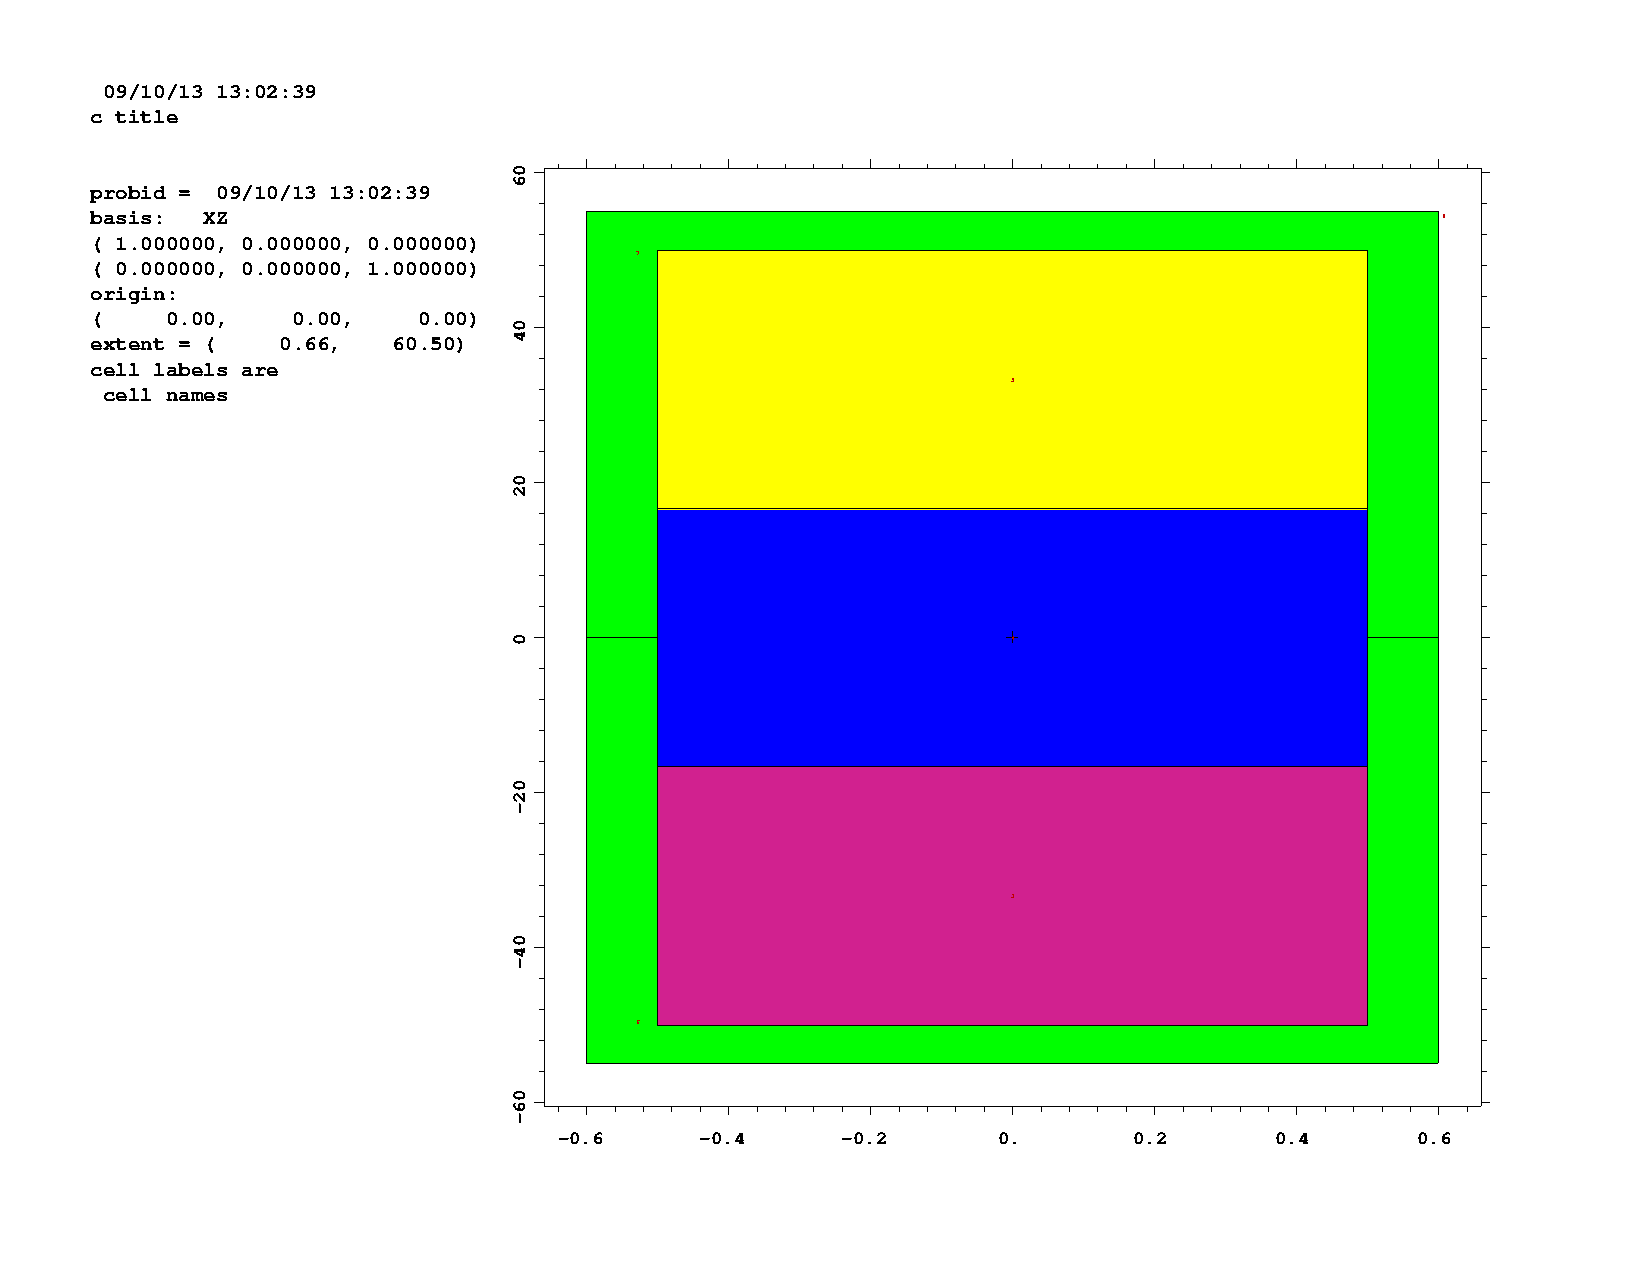
\includegraphics{i__p02.pdf}
\caption{Vertical section of MCNP model, plotted with MCNP. \label{pic:plot}}\end{figure}

Cell and surface numbers used in the input file are assigned automatically by
the MCNP interface, so that a user does not need to invent them and check their
uniqueness.

Density and temperature axial distributions are represented as a
set of cells with different density iand filled with different materials.
One can see three U-O mixtures, \code{m1}, \code{m2} and \code{m3} that represent the
same fuel isotopic composition but use different data suffixes. If there is no
cross-section data set prepared for a given temperature, it is interpolated
using two data sets with temperatures below and above the specified value, see
material \code{m2}. This technique is reffered to as pseudo-material cross-section
interpolation and is used for different type of reactors
\cite{pseudoMat2008,pseudoMatAlHamry}.  Note that we didn't
specify cross-section suffixes in the code above. Their choice depends on the
\code{\$DATAPATH} environmental variable (must be set before using PIRS), name of
the xsdir file (\code{xsdir} by default) and by material temperatures. When a
material is specified to the MCNP interface, it looks in the xsdir files for
the cross-sections with the closest temperature and correspondingly chooses the
suffix.

Mesh tallies are used to compute axial distribution of heat. Mesh tally parameters
are defined by the geometry element dimensions and its \code{heat} attribute. In
the example, the mesh tally covers a region that coincides with the fuel
cylinder and has ten axial equidistant mesh elements.


\subsection{High-level interface to SCF}
\label{paper:high-level-interface-to-scf}
The SCF code interface can handle only particular types of geometries described
by the general model classes. This limitation is due to the origin of problems
solved with SCF. Particularly, the general model defined above,  \code{b}, cannot be
handled with the current implementation of the SCF interface, since it needs a
model representing at least one rod -- a set of two or three coaxial cylinders
representing clad, gap and fuel regions of a rod. Thus the usage of the SCF
interface will be shown only schematically:

\begin{Verbatim}[commandchars=\\\{\}]
\PYG{k+kn}{from} \PYG{n+nn}{hpmc} \PYG{k+kn}{import} \PYG{n}{ScfInterface}

\PYG{n}{s} \PYG{o}{=} \PYG{n}{ScfInterface}\PYG{p}{(}\PYG{n}{r}\PYG{p}{)}

\PYG{c}{\PYGZsh{} ...}

\PYG{n}{s}\PYG{o}{.}\PYG{n}{inlet\PYGZus{}temperature} \PYG{o}{=} \PYG{l+m+mi}{560} \PYG{c}{\PYGZsh{} K}
\PYG{n}{s}\PYG{o}{.}\PYG{n}{total\PYGZus{}power} \PYG{o}{=} \PYG{l+m+mf}{3e4} \PYG{c}{\PYGZsh{} W}
\PYG{n}{s}\PYG{o}{.}\PYG{n}{inlet\PYGZus{}flow\PYGZus{}rate} \PYG{o}{=} \PYG{l+m+mi}{400} \PYG{c}{\PYGZsh{} g/s}
\PYG{n}{s}\PYG{o}{.}\PYG{n}{exit\PYGZus{}pressure} \PYG{o}{=} \PYG{l+m+mf}{15.5e6} \PYG{c}{\PYGZsh{} Pa}

\PYG{n}{p} \PYG{o}{=} \PYG{n}{s}\PYG{o}{.}\PYG{n}{run}\PYG{p}{(}\PYG{l+s}{\PYGZsq{}}\PYG{l+s}{R}\PYG{l+s}{\PYGZsq{}}\PYG{p}{)}
\end{Verbatim}

The usage of the SCF interface is similar to the usage of the MCNP interface.
First, an instance of the \code{ScfInterface} is created , its constructor takes a
general model as an argument. Additionally one needs to specify parts of the
general model representing fuel rods and optionally -- the part representing a
container (coolant channel wrapper).

In the current implementation, there are rather simplified possibilities to
specify boundary conditions. One can specify inlet temperature, total power,
inlet flow rate, exit pressure and some other (the SCF code has more
possibilities to specify boundary and initial conditions, for example one can
set inlet temperature to each subchannel).

Similar to the MCNP interface, the SCF code is started by calling the \code{run}
method of the interface. The SCF input file is generated, based on the geometry
information from the general model and SCF-specific data provided to the SCF
interface, the code is executed, and results -- fuel temperature, coolant
temperature and densities -- are read and returned in the general model copy.


\section{Example results for PWR assembly}
\label{paper:example-results-for-pwr-assembly}

\subsection{Assembly model}
\label{paper:assembly-model}
At the current stage, the MCNP and SCF interfaces allow to model a
assembly-like geometries.  Test calculations have been performed for a PWR
assembly  model based on the PWR benchmark specifications
\cite{PWRbenchmark}.

The assembly contains 264 UOX fuel pins and 25 guide tubes, positioned in a
square 17x17 lattice with 1.26 cm pitch; the model's horizontal cross-section
is a square with sides 21.42 cm. The model's height of 408.6 cm is defined by
the active length of fuel pins, plus lower and upper water reflectors, each
21.42 cm thick.  There are  two types of fuel pins: usual pins and pins with
IFBA (integrated fuel burnup absorber).

The coolant inlet temperature is 560 K. This temperature and correspondent
density (0.752 g/cm3 at 15.5 MPa) is used for the lower reflector.
Temperature and density of water in guide tubes is 580 K and 0.712 g/cm3,
respectively. The fuel and coolant in the active length region are divided into
11 axial layers of varying thickness to represent the fuel temperature, coolant
density and coolant temperature axial distributions. In the upper reflector,
the coolant properties are heterogeneous and correspond to the channel exit
parameters, as calculated by SCF.

All fuel pins have the same fuel composition: UO2 with U enriched to 4.2 \% (in
mass). The pin cladding and guide tube wall are represented by zircaloy-2 \cite{PWRbenchmark}.
Coolant is pure water. Gaps in fuel pins are filled with oxygen. The IFBA pins
have additional cylindrical layer of zirconium diboride (ZrB2).

In the MCNP models, in the active length region and in the upper reflector, the
coolant temperature and density as well as the fuel temperature are defined by
the SCF calculations. In the SCF models, the power profile is based on the MCNP
results.
\begin{figure}[htbp]
\centering
\capstart

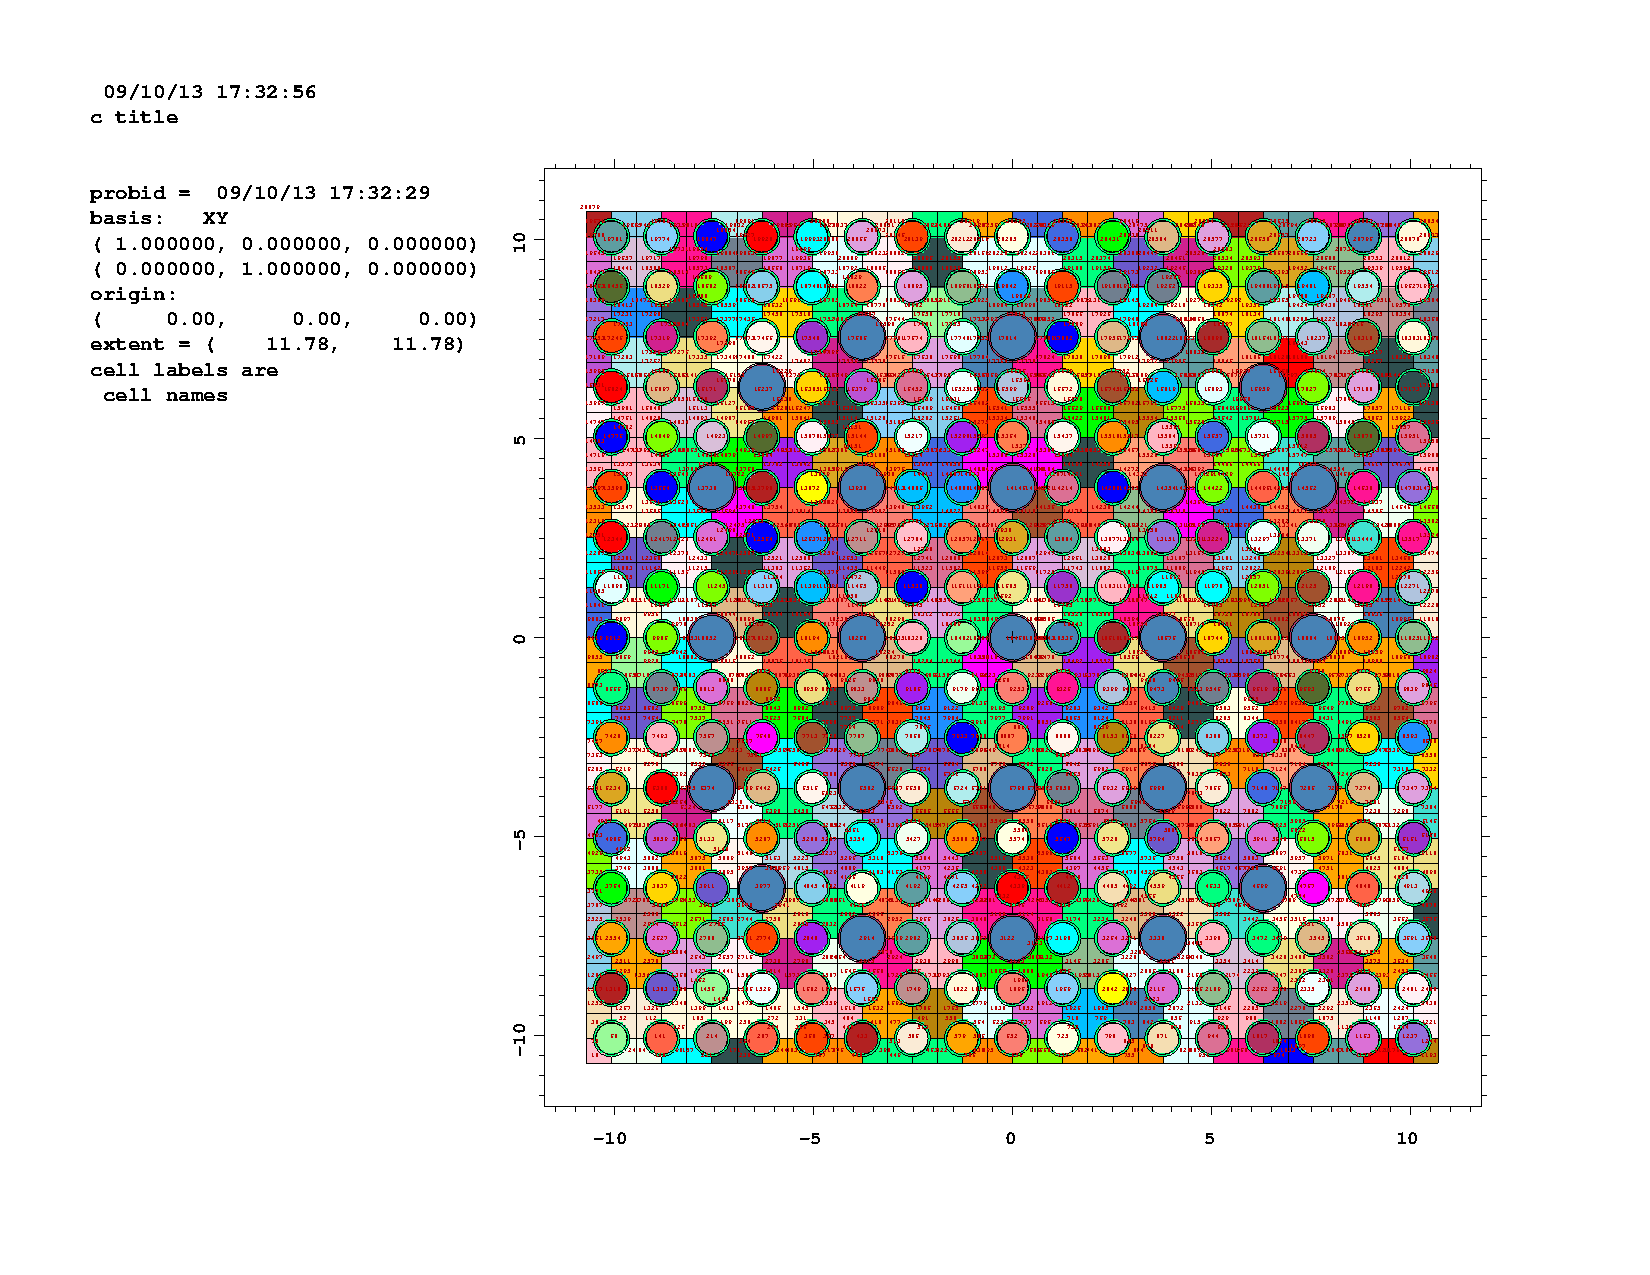
\includegraphics{i__p01.pdf}
\caption{Horizontal section of MCNP model at iteration 62. Different colors
correspond to materials with different temperatures.
\label{pic:hor}}\end{figure}
\begin{figure}[htbp]
\centering
\capstart

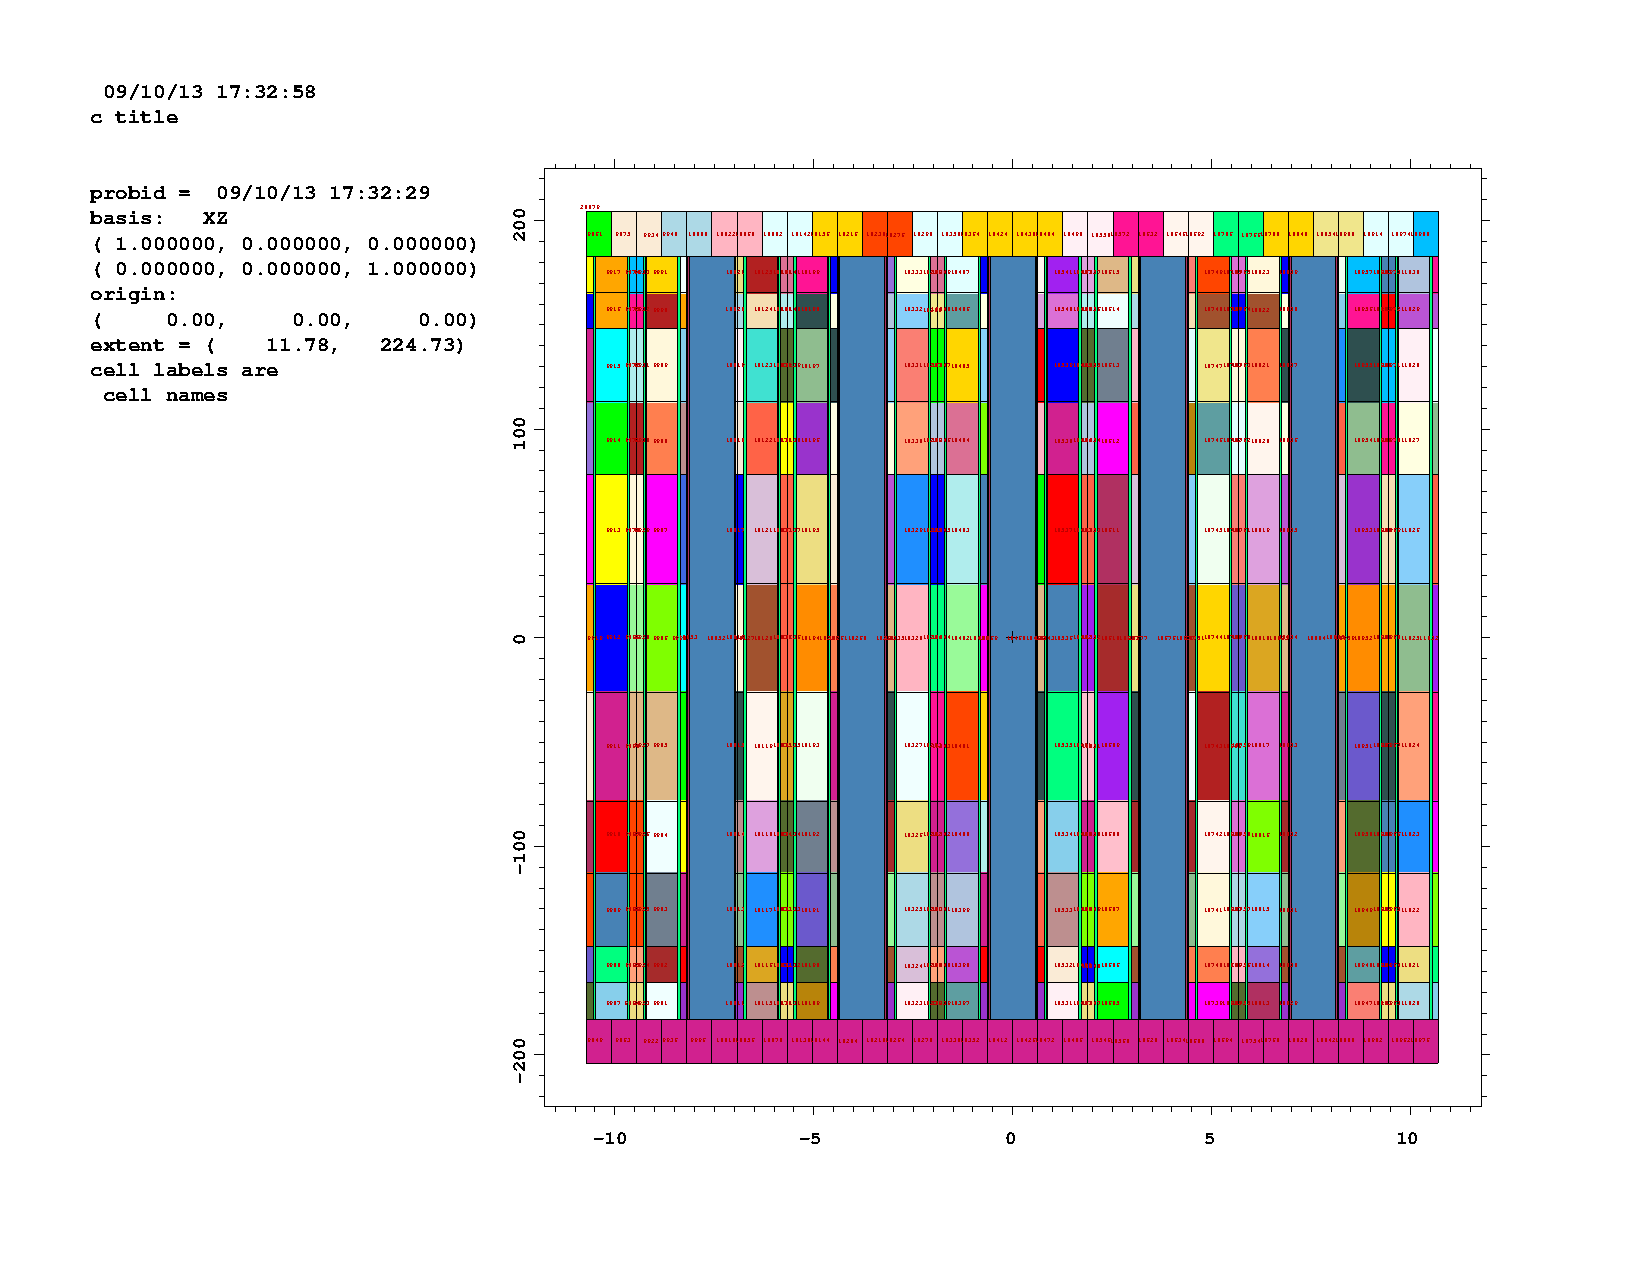
\includegraphics{i__p021.pdf}
\caption{Vertical section of MCNP model at iteration 62. \label{pic:ver}}\end{figure}

Figures \ref{pic:hor} and  \ref{pic:ver} show MCNP
plots for the model. The plots illustrate some capabilities of the MCNP and SCF
interfaces:
\begin{itemize}
\item {} 
the active length region can be split into axial layers arbitrarily;
in the assembly model we apply a non-uniform pattern with thiner layers at
the bottom and top of the model. The non-uniform pattern should represent a
cosine-like distribution of power density axial profile more accurately.

\item {} 
Subchannels in SCF are ``coolant-centered''. The subchannels are converted
into the MCNP model exactly, thus no interpolation or averaging of coolant
properties is necessary.

\item {} 
Bundle of pins is represented in the MCNP model using the lattice cell.
Another way to represent bundles of rods, without lattice cells, is also
implemented in the MCNP interface, but cannot be applied to a model with
17x17 elements.

\end{itemize}

The following boundary conditions are specified for SCF models: the coolant
inlet temperature is 560 K in all subchannels. Assembly thermal power is 18.47
MW; this value is obtained by dividing the core thermal power to the number of
assemblies in the core. The inlet mass flow rate is 82.12 kg/s; this value is
obtained also by dividing the average core mass flow rate to the number of
assemblies. The exit pressure is set to 15.5 MPa.

Thermo-physical properties of cladding and fuel pellets, specified in the
benchmark, are hard-coded in the SCF code under the name \code{'benpwr'}. These
properties are applied in the SCF calculations to compute fuel temperature.

The relaxation scheme \cite{dufek2006} is applied for the
coupled calculations. This scheme assumes an increase of statistical precision of
the MCNP results on each iteration. This is implemented by increasing the number of cycles. On
the first iteration, MCNP sampled 50 cycles with 1000 histories per cycle and
skipped first 10 cycles. On the 32-th iteration, MCNP sampled 835 cycles and on
the 62-nd iteration, MCNP sampled 1673 cycles.

For the demonstration calculations we have chosen an xsdir
with cross-sections sets for only two temperatures, 300 K and 1800 K (suffixes
31c and 40c, respectively). Thus, any fuel temperature is represented by a
mixture of only these two data sets, that minimizes the initialization time for
MCNP. To perform calculations with a finer cross-section temperature mesh, one
needs only to provide an xsdir with more data sets; no modifications in the
scripts describing the coupled calculations are needed.

The fuel temperature passed from SCF to MCNP is the radially-averaged
temperature, reported in the SCF output file in tables with rod results in the
column named \code{tfuave}.

The subchannel coolant temperature and density is reported by SCF at the
boundaries of each axial layer. Coolant parameters for MCNP models must
correspond to the layer interior, they are estimated as a mean of the boundary
values.


\subsection{Results}
\label{paper:results}
Results are shown for the 62-nd iteration. The coupled calculation has been
started with the convergence criterion set to 50 pcm, and should
iterate until the standard deviation of the value of Keff computed with MCNP, and the
difference between two values of Keff computed on subsequent iterations, become
below this value. At the 62-nd iteration, the convergence criterion is not meet yet,
iterations continue, but the intermediate results can be analyzed since all
necessary data is dumped after each iteration and can be processed without
stopping the iterations.

Figure \ref{pic:keff} shows Keff obtained on each cycle. In the
first iteration, the coolant properties correspond to an uniform power profile
and the initial neutron source is axially positioned in the center of the
assembly. These two aspects lead to a larger Keff, as compared to results
obtained on subsequent iterations. The statistical precision of Keff is
improved with iterations, since the number of sampled cycles in increased.
\begin{figure}[htbp]
\centering
\capstart

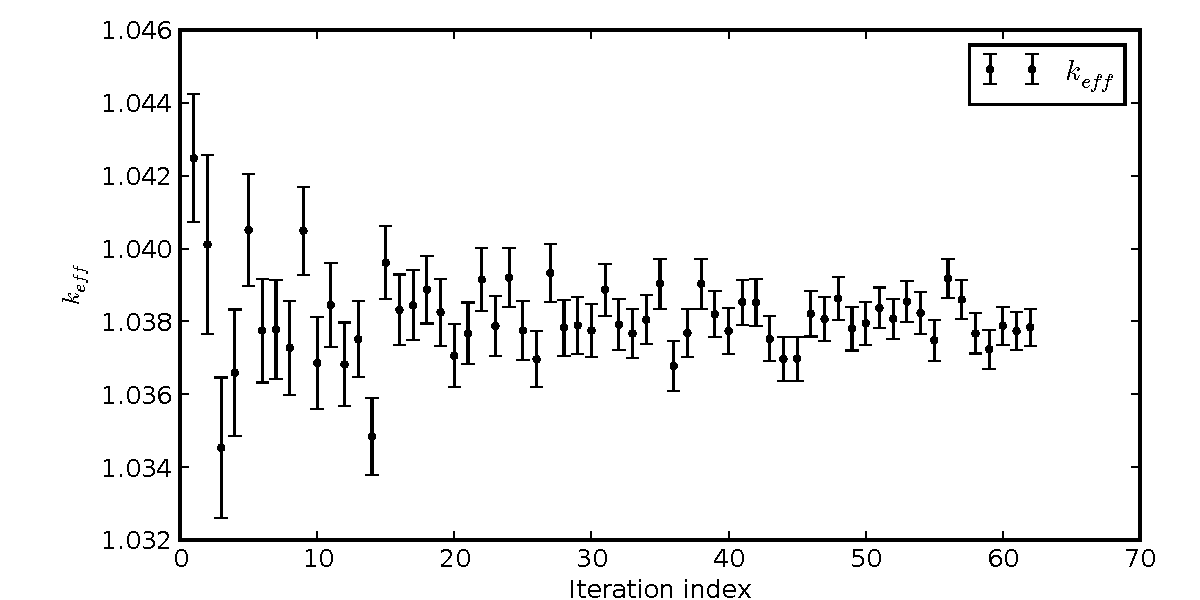
\includegraphics{b_iteration_062_keff.pdf}
\caption{Value of Keff versus iteration number. \label{pic:keff}}\end{figure}
\begin{figure}[htbp]
\centering
\capstart

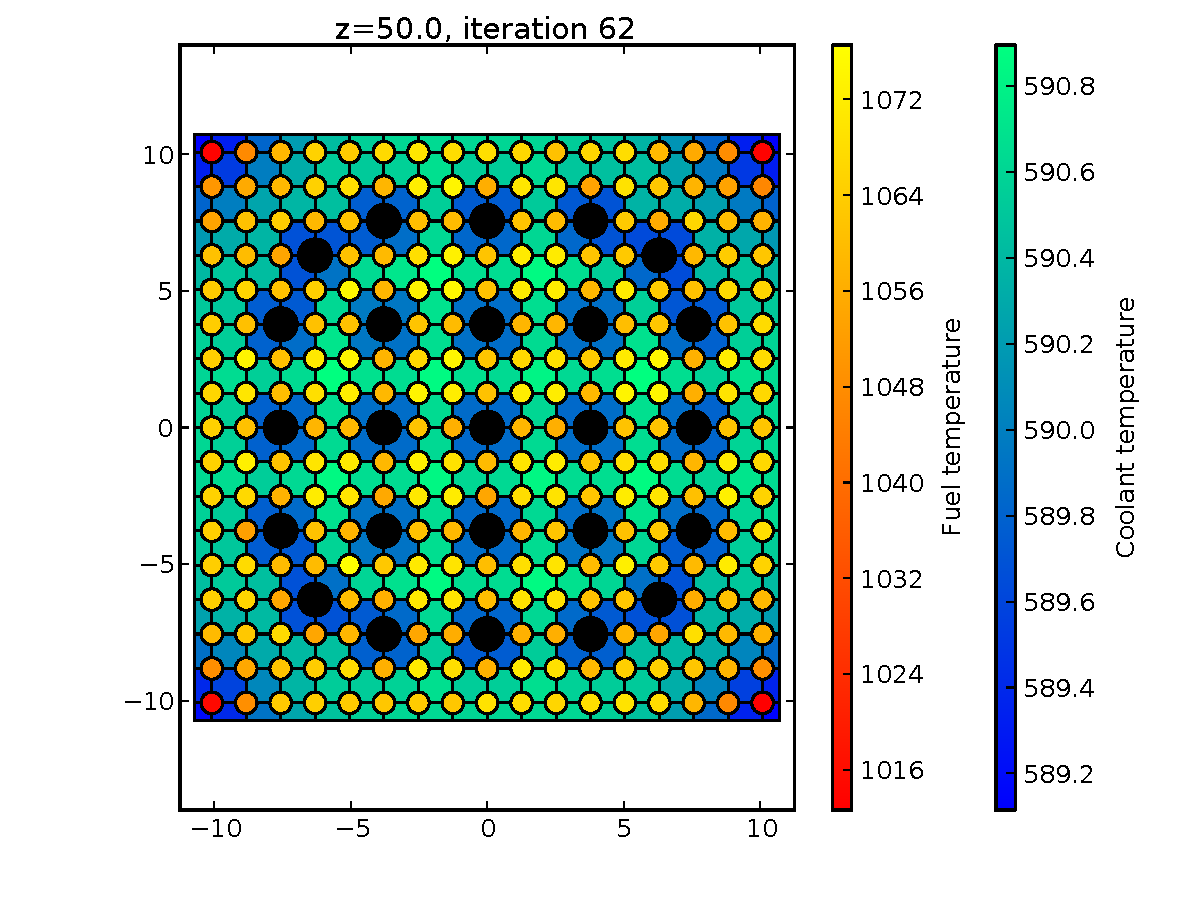
\includegraphics{b_iteration_062_temp50_0.pdf}
\caption{Coolant and fuel pellets temperature map in axial layer where maximal fuel
temperature is reached. \label{pic:tmap}}\end{figure}
\begin{figure}[htbp]
\centering
\capstart

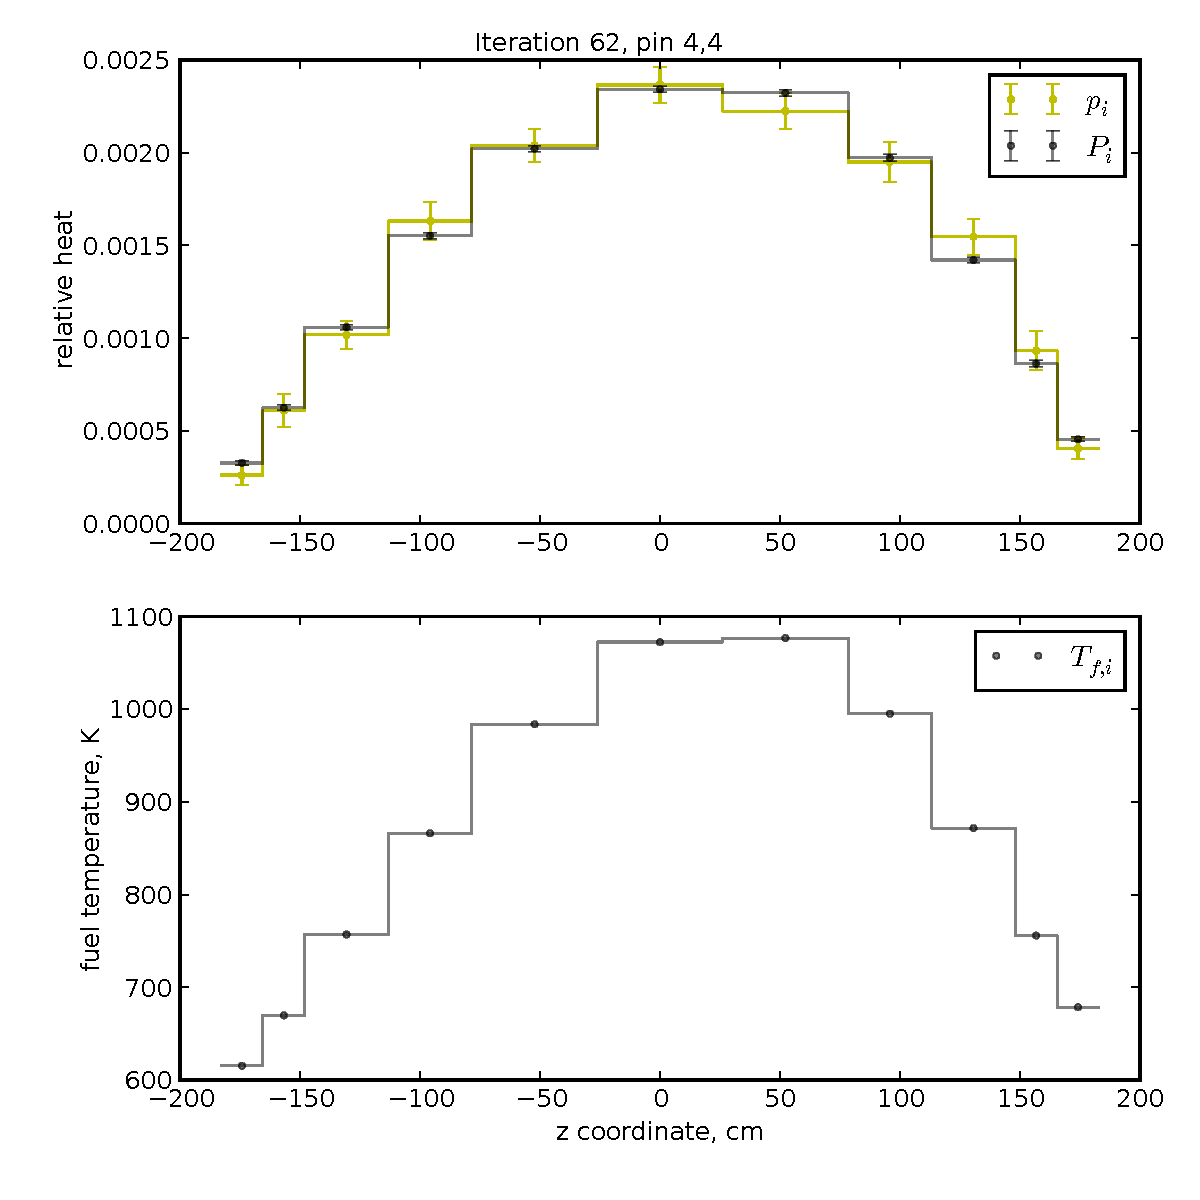
\includegraphics{b_iteration_062_4_4.pdf}
\caption{Axial distribution of power density and fuel temperature in the pin with
maximal power density. \label{pic:axial}}\end{figure}

The map on figure \ref{pic:tmap} shows radial temperature distribution of
fuel pellets and coolant. Although radial temperature
deviations are small, one can clearly see the effect of moderator channels to
the coolant temperature in adjacent channels.

The fuel temperature and power density axial distributions are shown on figure
\ref{pic:axial} for the fuel pin where the maximal power density
and maximal fuel temperature are reached. In the upper plot, the yellow line
shows results of the MCNP calculation on the 62-nd iteration and the black
line shows distribution of the relaxed power density. The later is used to get
fuel temperature axial distribution, which is shown on the lower plot on figure
\ref{pic:axial}.


\section{Current state  and outlook}
\label{paper:current-state-and-outlook}
At the current stage of development, PIRS provides a convenient way to setup
MCNP and SCF calculations for pin- and assembly-like geometries. The example
considered in the paper illustrates that description of a neutronics and TH
model using PIRS classes is more compact as compared to the correspondent input
files but still allows to set all relevant parameters.

The concept of PIRS -- independent description of geometry, and code interfaces that understand this
description -- establishes basis for coupled calculations. So far a code interface is added to PIRS,
it can be used to organize data transfer between this code and already integrated into PIRS.

Python runs on Windows, Linux/Unix and other OS \cite{pythonWEB}. Currently, PIRS has been
tested on desktop computers running Windows and Linux and on the JUQUEEN
supercomputer \cite{juqueenWEB}. Most of the PIRS code is OS-independent;
for OS-dependent parts of the code, Python has well-documented libraries.

Packages provided by the Python community simplify to large extent
post-processing of results obtained with PIRS. The code examples shown in this
paper illustrate only calculations-relevant part of PIRS. There are also
auxiliary classes and functions to dump calculation results for later use, to
generate plots etc. This allows to setup calculation work-flow starting from
input data specifications and up to generation of plots with results in a single
Python script.

PIRS documentation is written in parallel with the code itself, with a delay
necessary to avoid documenting of experimental stuff. The Sphinx
\cite{sphinxWEB} system is used. It provides environment, where
code examples -- very important part of software documentation -- is simple to
add and to keep updated with permanently developing software.

The presented framework, although already can be used to perform coupled
simulations of a pin- or assembly model, is under further development. The
nearest plans are dictated to large extent by the goals of the HPMC project.
Among them is ability to communicate with the job submission system of JUQUEEN,
which will allow to choose MCNP job parameters dependent on current loading of
the supercomputer. We also plan an interface to the SERPENT code
\cite{serpentWEB}.  Futher plans might include interfaces to the
KANEXT \cite{kanext} system developed at our institute; this
however lies beyond the HPMC project.


\section{Acknowledgment}
\label{paper:acknowledgment}
This work is funded by the European Commission via the FP7 project HPMC
``High-Performance Monte Carlo Reactor Core Analysis'' under contract no. 295971.
\bibliography{hpmc}
\bibliographystyle{ans}


\renewcommand{\indexname}{Index}

\end{document}
